\Chapter{System Architecture}

\section{Overview}
This application uses HTTPS exclusively for security reasons, except in the local developer environment, where we use unencrypted HTTP, as shown in Figure ~\ref{fig:deployment}.

\vspace{3em}
\begin{figure}[H]
\begin{center}
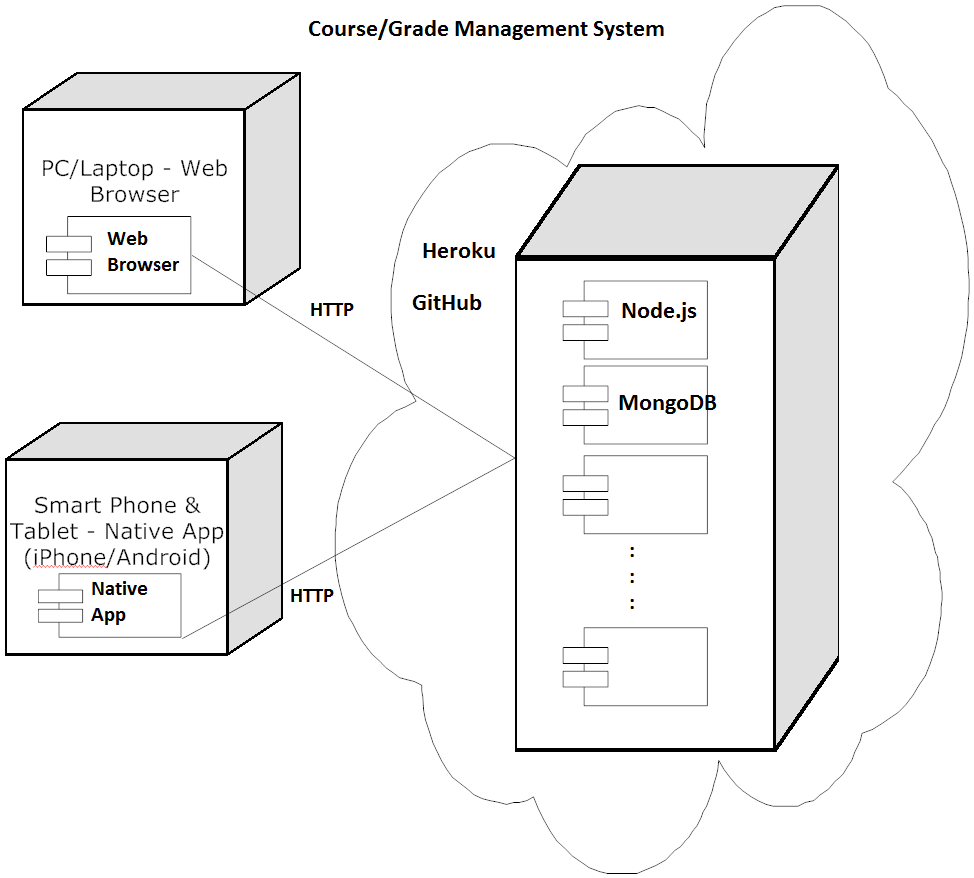
\includegraphics[height=3.8in,width=6.5in]{images/deployment.png}
\caption{Deployment Diagram}
\label{fig:deployment}
\end{center}
\end{figure}

\section{Deployment Workflow}
There are three type of environments used in the deployment workflow: development, staging and production. Figure ~\ref{fig:system-integration} illustrates the deployment workflow.

\vspace{3em}
\begin{figure}[H]
\begin{center}
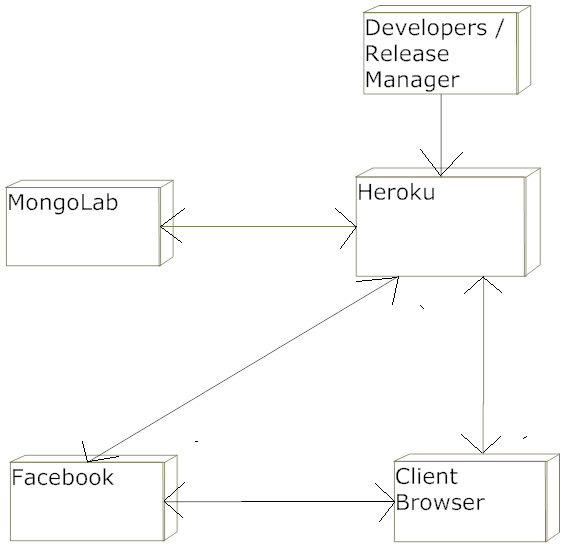
\includegraphics[height=3.8in,width=6.5in]{images/systemIntegration.png}
\caption{System Integration}
\label{fig:system-integration}
\end{center}
\end{figure}

\begin{itemize}
\item Developers work on new features or bug fixes in development branches. Only minor updates are committed directly to the stable development branch.
\item Once features are implemented and/or set of bugs are fixed, they are merged in to staging branch and deployed to staging environment for testing and quality assurance
\item After testing is completed, the snapshop of staging branch is kept for production deployment, otherwise the process will repeat until the testing is completed.
\item On the release date, the working staging branch is deployed to production environment.
\end{itemize}

On this project, git is used as code repositories, to manage developments, staging and production branch. And Heroku toolbelt is also used to set the enviroment config variable for each deployment. Heroku allows users to use git to deploy automatically from local repositories. 
 
\section{Developer/Release}
In this project, developers first do unit testing in local machine, then after it reached certain point, developer himself or assign release manager use git to push the changes to staging or production repositories that connected to respective Heroku servers. 

Below are the command the developer/release manager uses to start the application, then commit and push the changes to remote repository.
\begin{lstlisting}
$ foreman start
18:43:16 web.1  : started with pid 5540
18:43:16 web.1  : listening on 5000
\end{lstlisting}

\begin{lstlisting}
$ git status
\end{lstlisting}

\begin{lstlisting}
$ git add .
\end{lstlisting}

\begin{lstlisting}
git commit -m "message here"
\end{lstlisting}

\begin{lstlisting}
$ git push master remote
$ git push staging remote
$ git push production remote
\end{lstlisting}


\section{Heroku}
In this project there are two sets of heroku instances used: staging and production. 
The application running in Heroku connects to a database server running inside MongoLab using the MongoDB protocol to read and/or write data to database.  Heroku also talks to Facebook servers via Facebook's Open Graph API.

Below are the sample of Heroku command to create staging environment and edit configuration variables
\begin{lstlisting}
$ heroku create --remote staging
\end{lstlisting}

\begin{lstlisting}
$ git config heroku.remote staging
\end{lstlisting}

\section{MongoLab}
In this project there are three sets of mongo databases used: development, staging and production. It is important to keep the versions of databases since new versions of changes may include changes in database structure, so rolling back or forward the application version would not cause any error. 

Below are the command how to connect to remote Mongo Database that hosted in MongoLab

\begin{lstlisting}
$ mongo <servername>.mongolab.com:<portno>/<dbname> 
-u <dbuser> -p <dbpassword>
\end{lstlisting}

\section{Facebook}
Facebook is playing an important role in this project. Facebook provides user authentication and social media integration. Facebook allows connection using the Facebook API and Open Graph API.

\section{Client Browser}
Client browser uses HTTPS GET for static content, and HTTPS POST for AJAX request to Heroku. And client browser also connects to Facebook server directly using Facebook API and Open Graph API in HTTPS.
 
